\documentclass[11pt]{article}
\usepackage[spanish]{babel}
\spanishdecimal{.}
\usepackage[utf8]{inputenc}
\usepackage[T1]{fontenc}
\usepackage[margin=2.2cm]{geometry}
\usepackage{amsmath,amssymb}
\usepackage{graphicx}
\usepackage{booktabs}
\usepackage{caption}
\usepackage{float}

\setlength{\parskip}{0.4em}
\setlength{\parindent}{0pt}

\title{\textbf{Tarea 1: Descripción y Análisis Exploratorio de Datos\\ Transformación Box--Cox}}
\author{Equipo: EAB Model}
\date{\today}

\begin{document}
\maketitle
\thispagestyle{empty}

\section*{Parte I. Descripción y Análisis Exploratorio de Datos}
\subsection*{Prestigio de la Ocupación en Canadá (Censo 1971)}

\subsubsection*{1. Análisis exploratorio}

El conjunto de datos contiene 102 ocupaciones canadienses, descritas por 7 variables: educación y ocupación promedio, ingreso promedio, porcentaje de mujeres, calificación de prestigio, código de censo y tipo de ocupación.

\begin{table}[H]
\centering
\caption{Estadísticos descriptivos de las variables cuantitativas continuas.}
\begin{tabular}{lrrrrr}
\toprule
Variable & Media & Mediana & Desv. Est. & Mín. & Máx. \\
\midrule
Educación (años) & 10.74 & 10.54 & 2.73 & 6.38 & 15.97 \\
Ingreso (\$) & 6798 & 5930 & 4246 & 611 & 25880 \\
Mujeres (\%) & 28.98 & 13.60 & 31.72 & 0.00 & 97.51 \\
Prestigio & 46.83 & 43.60 & 17.20 & 14.80 & 87.20 \\
\bottomrule
\end{tabular}
\end{table}

\begin{table}[H]
\centering
\caption{Frecuencias de la variable \texttt{tipo}.}
\begin{tabular}{lrr}
\toprule
Categoría & Frecuencia & Porcentaje \\
\midrule
Obrero (bc) & 44 & 43.1\% \\
Profesional (prof) & 31 & 30.4\% \\
Oficinista (wc) & 23 & 22.5\% \\
Sin clasificar (NA) & 4 & 3.9\% \\
\bottomrule
\end{tabular}
\end{table}

El análisis exploratorio reveló varios detalles relevantes. Primero, la variable \texttt{tipo} tiene 4 valores faltantes (Athletes, Newsboys, Babysitters, Farmers), ocupaciones que no encajan en ninguna de las tres categorías del esquema Pineo-Porter. Segundo, la variable \texttt{mujeres} está fuertemente polarizada, con una alta concentración de ocupaciones cerca de 0\% y cerca de 100\% de participación femenina, reflejando la marcada segregación ocupacional por género en 1971. Tercero, se identificaron dos observaciones casi idénticas, Slaughterers.1 y Slaughterers.2, con el mismo código de censo y los mismos valores de educación, ingreso y porcentaje de mujeres, pero con prestigio distinto (25.2 vs.\ 34.8) --- probablemente corresponden a la misma ocupación evaluada en dos momentos o grupos distintos del estudio original. Finalmente, aunque el rango de \texttt{ingreso} (de 611 a 25{,}879) no representa un comportamiento anómalo, la media (6798) está considerablemente por encima de la mediana (5930) debido a un valor extremo en el percentil 100; para fines descriptivos, la mediana sería una medida de tendencia central más robusta, aunque no hay justificación para excluir dicha observación del análisis.

\subsubsection*{2. Clasificación de variables}

\begin{table}[H]
\centering
\caption{Clasificación de las variables del conjunto de datos.}
\begin{tabular}{ll}
\toprule
Variable & Clasificación \\
\midrule
Ocupación & Cualitativa (nominal) --- identificador único por observación \\
Educación & Cuantitativa continua --- nivel educativo promedio \\
Ingreso & Cuantitativa continua --- ingreso promedio \\
Mujeres & Cuantitativa continua --- porcentaje de mujeres \\
Prestigio & Cuantitativa continua --- calificación de prestigio \\
Censo & Cualitativa (nominal) --- código de la ocupación en el censo \\
Tipo & Cualitativa (nominal) --- obrero / profesional / oficinista \\
\bottomrule
\end{tabular}
\end{table}

Educación, ingreso, mujeres y prestigio son cuantitativas continuas, ya que son promedios o porcentajes que pueden tomar cualquier valor real dentro de un rango (aunque ingreso se observe en números enteros, es un promedio, no una medición individual). Censo y ocupación, aunque se ven como número y texto respectivamente, son etiquetas identificadoras, no magnitudes --- son cualitativas nominales, al igual que tipo. No hay ninguna variable cuantitativa discreta en este conjunto de datos.

\subsubsection*{3. Prestigio vs. nivel educativo}

\begin{figure}[H]
\centering
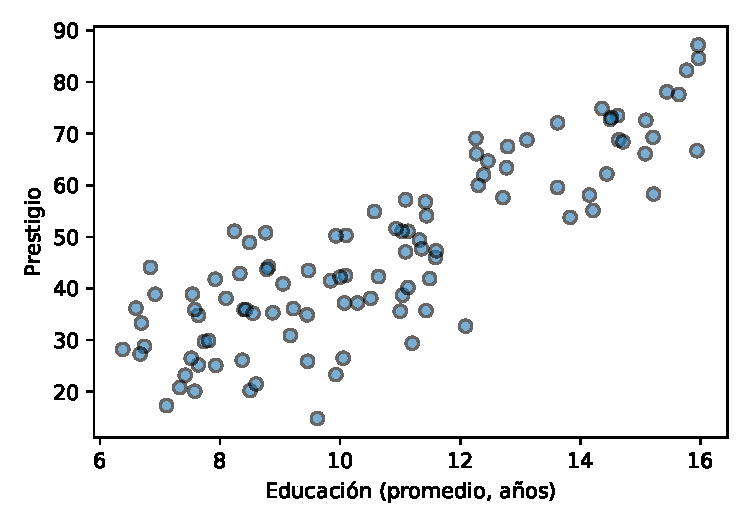
\includegraphics[width=0.55\textwidth]{fig1.pdf}
\caption{Prestigio vs. nivel educativo.}
\end{figure}

Se identifica una relación positiva y fuerte entre el nivel educativo y el prestigio de la ocupación (coeficiente de correlación de Pearson $r=0.8502$, cercano a 1). La Figura 1 confirma esta tendencia: a mayor nivel educativo promedio, mayor prestigio en promedio, aunque con cierta dispersión alrededor de la tendencia (ocupaciones con niveles educativos similares pueden tener prestigios distintos).

\section*{Parte II. Transformación Box--Cox}
\subsection*{Consumo de electricidad vs. consumo de agua}

\subsubsection*{a. Datos originales}

\begin{figure}[H]
\centering
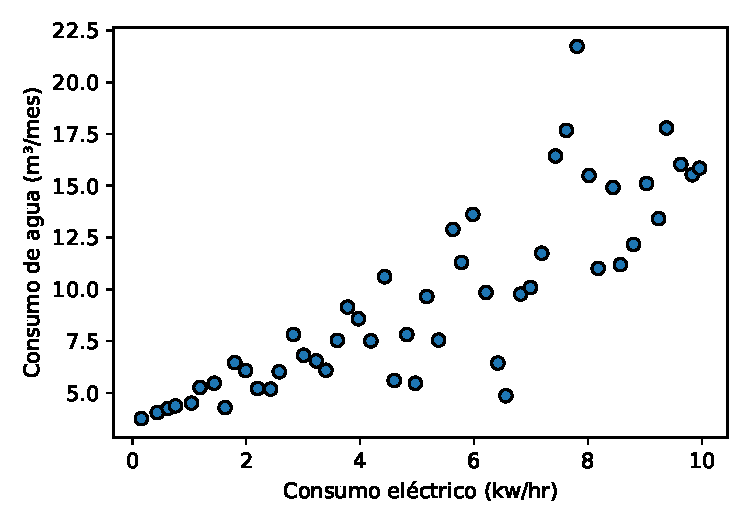
\includegraphics[width=0.55\textwidth]{fig2.pdf}
\caption{Consumo de agua vs. consumo eléctrico.}
\end{figure}

Los datos muestran una tendencia aproximadamente lineal entre ambas variables, con una relación positiva: a mayor consumo eléctrico, mayor consumo de agua. No obstante, la dispersión de los puntos alrededor de esta tendencia no es constante --- conforme aumenta el consumo eléctrico, la variabilidad del consumo de agua también aumenta, lo cual sugiere un problema de heterocedasticidad que deberá confirmarse mediante el análisis de residuales.

\subsubsection*{b. Regresión lineal simple sobre los datos sin transformar}

Se ajusta el modelo $y_i = \beta_0 + \beta_1 x_i + \varepsilon_i$, con $\varepsilon_i \overset{iid}{\sim} N(0,\sigma^2)$, mediante mínimos cuadrados: $\hat\beta = (X'X)^{-1}X'y$.

\begin{table}[H]
\centering
\caption{Modelo de regresión lineal simple, datos sin transformar.}
\begin{tabular}{lrrrr}
\toprule
Parámetro & Estimador & Error Est. & $t$ & $p$ \\
\midrule
$\beta_0$ & 2.8841 & 0.707 & 4.081 & $<0.001$ \\
$\beta_1$ & 1.3023 & 0.121 & 10.805 & $<0.001$ \\
\bottomrule
\end{tabular}
\end{table}

Con $R^2=0.709$. Ambos coeficientes son altamente significativos.

\subsubsection*{c. Análisis de residuales}

Los residuales son $e_i=y_i-\hat y_i$. El modelo asume homocedasticidad, $\text{Var}(\varepsilon_i\mid x_i)=\sigma^2$ constante. La prueba de Breusch-Pagan contrasta $H_0$: varianza constante; la prueba de Jarque-Bera contrasta $H_0$: normalidad de los residuales.

\begin{figure}[H]
\centering
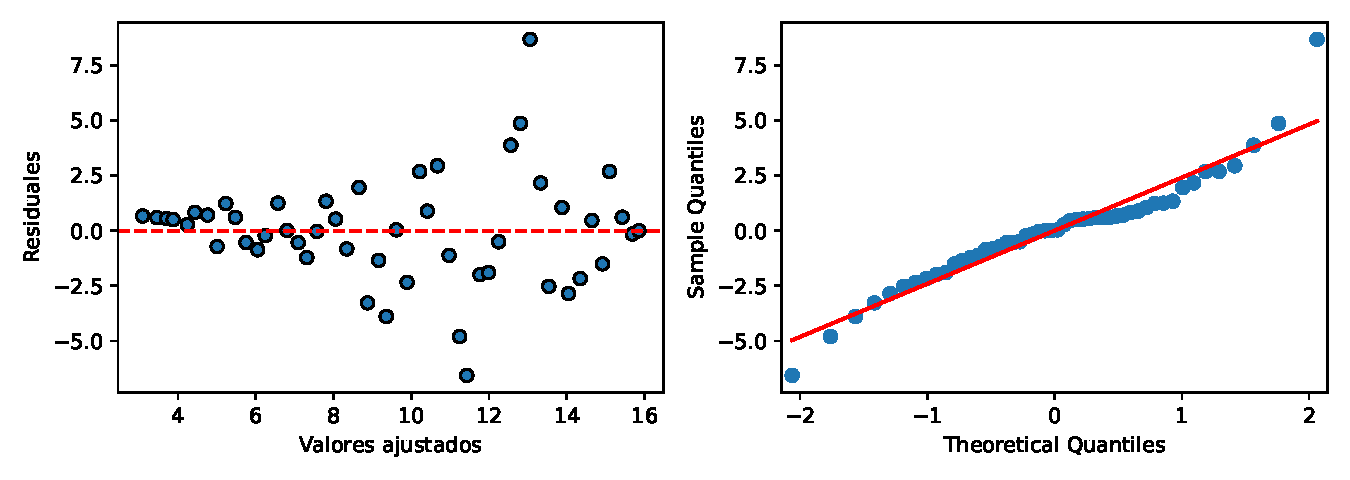
\includegraphics[width=0.85\textwidth]{fig3.pdf}
\caption{Diagnóstico de residuales del modelo sin transformar. (a) Residuales vs.\ valores ajustados; (b) QQ-plot de residuales.}
\end{figure}

En la Figura 3(a) se observa heterocedasticidad: conforme aumentan los valores ajustados, aumenta la varianza de los residuales, formando un patrón de abanico (Breusch-Pagan: estadístico$=3.835$, $p=0.0502$, en el límite de significancia). En la Figura 3(b) se observan dos outliers que impiden la normalidad en las colas (Jarque-Bera: $p=0.000174$). En conjunto, estas gráficas muestran que el modelo lineal sin transformar no es adecuado.

\subsubsection*{d. Transformación Box-Cox}

La transformación Box-Cox normalizada es
$$y^{(\lambda)} = \begin{cases} \dfrac{y^\lambda - 1}{\lambda\, \dot y^{\lambda-1}} & \lambda \neq 0 \\[6pt] \dot y \ln(y) & \lambda = 0 \end{cases}, \qquad \dot y = \left(\prod_{i=1}^n y_i\right)^{1/n}$$
Se ajusta $y^{(\lambda)} = \beta_0 + \beta_1 x + \varepsilon$ para distintos $\lambda$, y se elige $\hat\lambda = \arg\min_\lambda SC_{\text{Res}}(\lambda)$. El intervalo aproximado del $100(1-\alpha)\%$ de confianza para $\lambda$ es $\{\lambda : SC_{\text{Res}}(\lambda) \leq SC^*\}$, con
$$SC^* = SC_{\text{Res}}(\hat\lambda)\left(1 + \frac{t^2_{(1-\alpha/2,\,\nu)}}{\nu}\right), \qquad \nu = n-2$$

\begin{figure}[H]
\centering
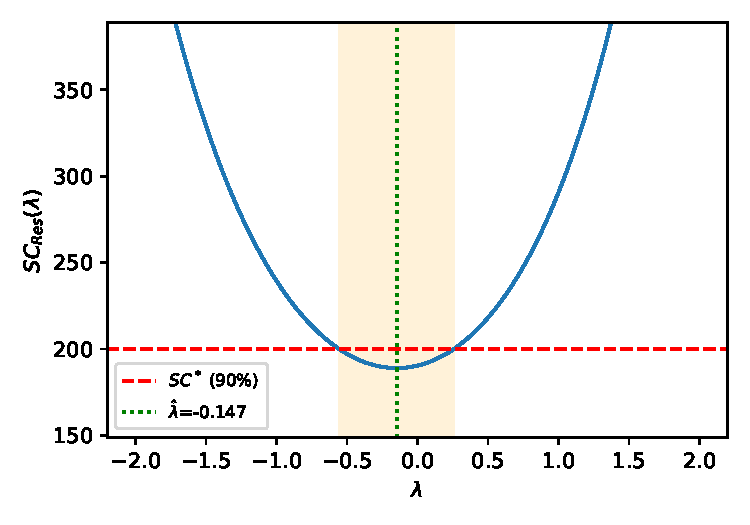
\includegraphics[width=0.55\textwidth]{fig4.pdf}
\caption{$SC_{\text{Res}}(\lambda)$ de la transformación Box-Cox.}
\end{figure}

Se obtuvo $\hat\lambda = -0.147$, con un intervalo de confianza del 90\% de $(-0.556,\ 0.258)$. Como $\lambda=0$ también está dentro de este intervalo ($SC_{\text{Res}}(0)=190.35$ vs.\ $SC_{\text{Res}}(\hat\lambda)=188.93$, ambos muy por debajo del umbral $SC^*=199.998$), y es más simple e interpretable que $-0.147$, se utiliza $\lambda=0$ (transformación logarítmica) para los siguientes incisos, sin que esto implique una pérdida de ajuste relevante.

\subsubsection*{e. Gráfica de la respuesta transformada}

\begin{figure}[H]
\centering
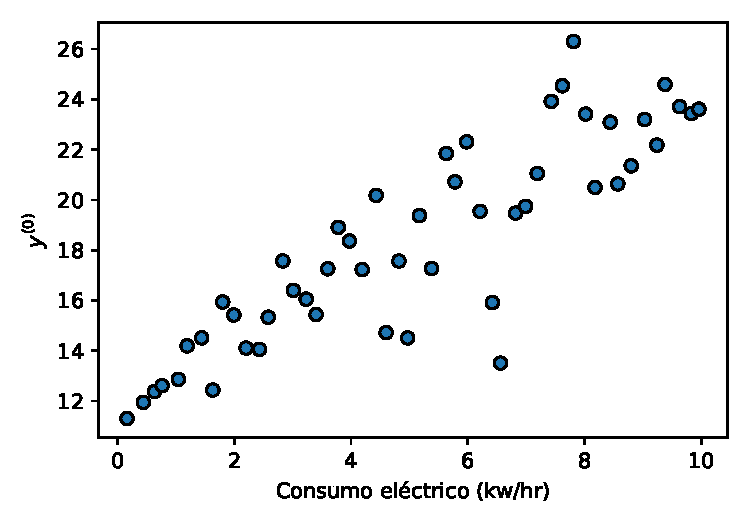
\includegraphics[width=0.55\textwidth]{fig5.pdf}
\caption{$y^{(\lambda)}$ vs.\ $x$, con $\lambda=0$.}
\end{figure}

La Figura 5 muestra que la transformación corrigió el problema de varianza creciente conforme aumenta $x$ observado en la Figura 2. Ahora la dispersión de los puntos se mantiene aproximadamente constante en todo el rango de $x$, tanto para valores chicos como para valores grandes.

\subsubsection*{f. Modelo transformado y validación}

Con $\lambda=0$ fijo se ajusta $y^{(0)}_i = \beta_0 + \beta_1 x_i + \varepsilon_i$, con $y^{(0)}_i = \dot y \ln(y_i)$.

\begin{table}[H]
\centering
\caption{Modelo de regresión sobre la respuesta transformada ($\lambda=0$).}
\begin{tabular}{lrrrr}
\toprule
Parámetro & Estimador & Error Est. & $t$ & $p$ \\
\midrule
$\beta_0$ & 12.1300 & 0.572 & 21.200 & $<0.001$ \\
$\beta_1$ & 1.2153 & 0.098 & 12.454 & $<0.001$ \\
\bottomrule
\end{tabular}
\end{table}

Con $R^2=0.764$ (mayor al 0.709 del modelo sin transformar).

\begin{figure}[H]
\centering
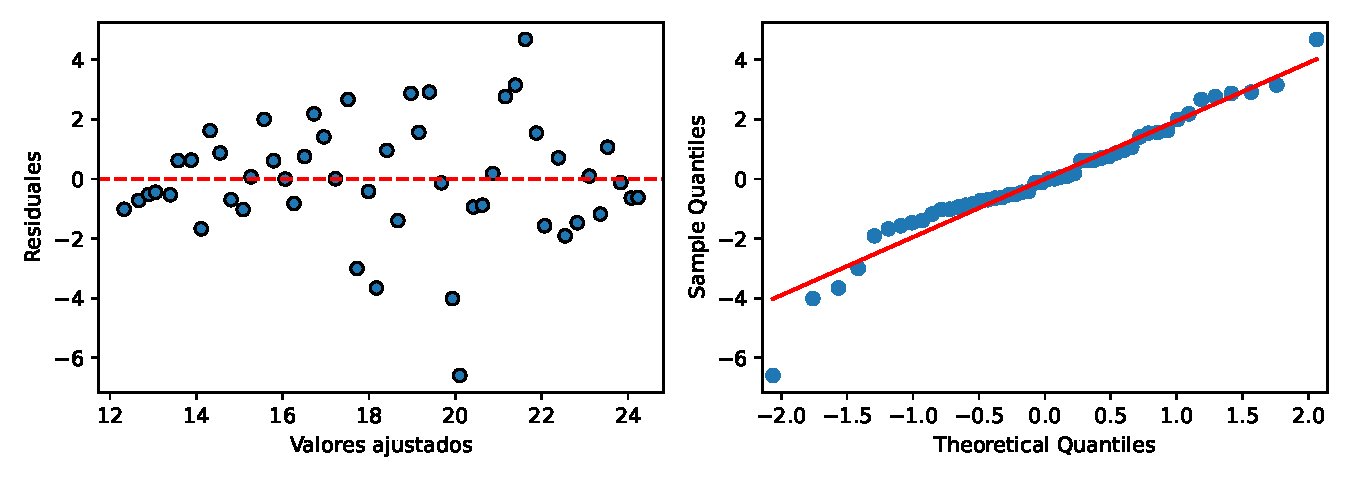
\includegraphics[width=0.85\textwidth]{fig6.pdf}
\caption{Diagnóstico de residuales del modelo transformado. (a) Residuales vs.\ valores ajustados; (b) QQ-plot de residuales.}
\end{figure}

La Figura 6(a) muestra una mejora notable en la homocedasticidad respecto a la Figura 3(a): la razón entre la dispersión de residuales en la mitad alta y la mitad baja de los valores ajustados se redujo de 2.6 a 1.8 veces, y la prueba de Breusch-Pagan pasó de un p-valor de 0.0502 a 0.2112, sin evidencia de heterocedasticidad en el modelo transformado. La normalidad también mejoró (Jarque-Bera: $p$ de 0.000174 a 0.0203), aunque sigue sin cumplirse plenamente al 5\%.

\begin{table}[H]
\centering
\caption{Observaciones con mayor residual absoluto.}
\begin{tabular}{lrrrr}
\toprule
Obs. & $x$ (elec.) & $y$ (agua) & Residual sin transf. & Residual transf. \\
\midrule
33 & 6.56 & 4.86 & $-6.568$ & $-6.593$ \\
39 & 7.81 & 21.73 & $8.680$ & $4.689$ \\
\bottomrule
\end{tabular}
\end{table}

Esto se explica por dos observaciones atípicas, presentes en ambos modelos. El residual de la observación 39 mejoró considerablemente (de 8.68 a 4.69), mientras que el de la observación 33 prácticamente no cambió, ya que corresponde a un dato genuinamente atípico que la transformación no puede corregir. En conjunto, la transformación Box-Cox mejoró sustancialmente el modelo, sin resolver por completo el problema de normalidad.

\subsubsection*{g. Intervalo de confianza del 90\% para el consumo medio de agua}

El intervalo de confianza del $100(1-\alpha)\%$ para la respuesta media $E[Y^{(0)}\mid x_0]$ es
$$\hat y_0^{(0)} \pm t_{(1-\alpha/2,\,n-2)} \cdot s\sqrt{\dfrac{1}{n} + \dfrac{(x_0-\bar x)^2}{S_{xx}}}$$
Con $x_0=7.57$ y $\alpha=0.10$. El intervalo se calcula en la escala transformada y se invierte con $y=\exp(y^{(0)}/\dot y)$, válido porque la transformación es monótona.

\begin{figure}[H]
\centering
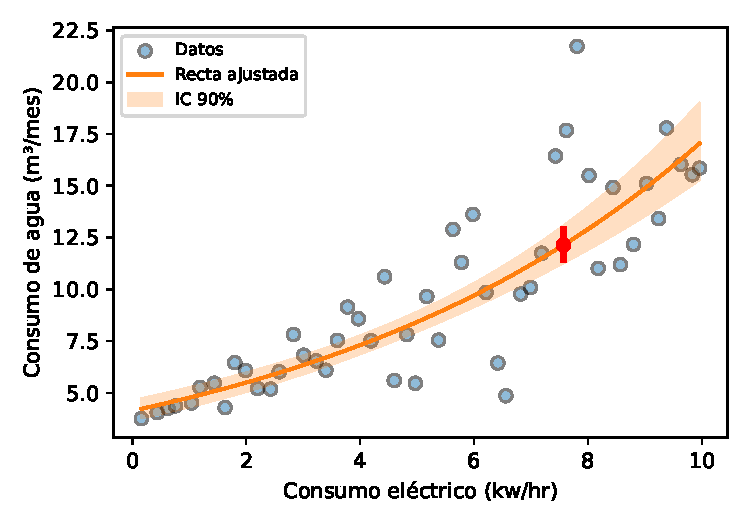
\includegraphics[width=0.55\textwidth]{fig7.pdf}
\caption{Intervalo de confianza del 90\% para el consumo medio de agua, escala original.}
\end{figure}

Con 90\% de confianza, el consumo medio de agua esperado para un consumo eléctrico de 7.57 kw/hr está entre \textbf{11.284 y 13.050 m$^3$/mes} (estimación puntual: 12.135 m$^3$/mes).

\subsubsection*{h. Intervalo de predicción del 95\% para el consumo de agua}

El intervalo de predicción para una observación individual nueva $Y_{\text{nuevo}}\mid x_0$ es
$$\hat y_0^{(0)} \pm t_{(1-\alpha/2,\,n-2)} \cdot s\sqrt{1 + \dfrac{1}{n} + \dfrac{(x_0-\bar x)^2}{S_{xx}}}$$
Con $x_0=5.1$ y $\alpha=0.05$. La diferencia con la fórmula del inciso (g) es el ``+1'' dentro de la raíz: incorpora la varianza de una observación individual alrededor de la recta, además de la incertidumbre de estimar la recta misma.

\begin{figure}[H]
\centering
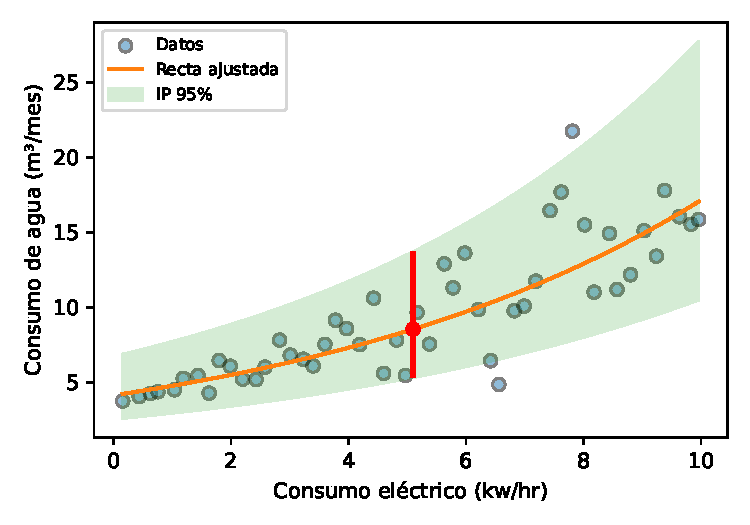
\includegraphics[width=0.55\textwidth]{fig8.pdf}
\caption{Intervalo de predicción del 95\% para una observación individual, escala original.}
\end{figure}

Con 95\% de confianza, el consumo de agua de una observación individual con consumo eléctrico de 5.1 kw/hr estará entre \textbf{5.321 y 13.709 m$^3$/mes} (estimación puntual: 8.541 m$^3$/mes). La Figura 8 es mucho más ancha que la Figura 7 porque esta última es un intervalo de predicción, con varianza más alta por tratarse de un punto individual, mientras que la Figura 7 es un intervalo de confianza para el consumo ``medio''.

\end{document}
